
%\documentclass[calculator,allquestions,datasheet,solutions]{exam_newMarcus2}
\documentclass[calculator,allquestions,datasheet,Pens]{exam_newMarcus2}

% The full list of class options are
% calculator : Allows approved calculator use.
% datasheet : Adds a note that data sheet are attached to the exam.
% handbook : Allows the use of the engineering handbook.
% resit : Adds the resit markings to the paper.
% sample : Adds conspicuous SAMPLE markings to the paper
% solutions : Uses the contents of \solution commands (and \solmarks) to generate a solution file

\usepackage{pdfpages}  
\usepackage{lscape,comment} 
 
\coursecode{EX3029}%% 
\coursetitle{Chemical Thermodynamics}
 
\examtime{00.00--00.00}%
\examdate{15}{12}{2017}% 
\examformat{Attempt ALL questions. \\ Each question is worth 20 marks.}

% Other symbols
\newcommand{\frc}{\displaystyle\frac}
\newcommand{\br}[1]{\!\left( #1 \right)}
\newcommand{\abs}[1]{\left| #1 \right|}
\newcommand{\fracd}[2]{\frac{\mathrm{d} #1}{\mathrm{d} #2}}
\newcommand{\fracp}[2]{\frac{\partial #1}{\partial #2}}
\renewcommand{\d}[1]{\mathrm{d} #1 } 
\newcommand{\Ma}{\mathrm{M\!a}} 
\newcommand{\eg}{{\it e.g., }}
\newcommand{\ie}{{\it i.e., }}
\newcommand{\wrt}{{\it wrt }}
\newcommand{\Partial}[3][error]{\left(\frc{\partial #1}{\partial #2}\right)_{#3}}
\newcommand{\mfr}[3][error]{#1_{#2}^{\left(#3\right)}} 
\newcommand{\summation}[3][error]{\sum\limits_{#2}^{#3}#1}


\begin{document}


%%%
%%% Question 01 
%%%
\begin{question}
   An engineering consultancy company is contracted to design a separation process for a mixture of petroleum naphtha and fertilisers by-products. The mixture will be separated by a series of distillation and crystallisation processes. After the first distillation, lighter and heavier streams are stored in two pressure vessels:
         \begin{itemize}
            \item {\bf Vessel 1:} 45 mol-$\%$ of n-hexane, 30 mol-$\%$ of n-heptane and 25 mol-$\%$ of i-octane;
            \item {\bf Vessel 2:} 1.70 mol-$\%$ of n-hexane  and 98.30 mol-$\%$ of chlorobenzene.
         \end{itemize} 
         Vessels 1 and 2 are kept at 1.5 and 4.5 bar, respectively. In order to design the second set of distillations, 
         \begin{enumerate}[a)]
            \item  Estimate the bubble and dew temperatures for Vessel 1. Also calculate the compositions at bubble and dew points;~\marks{9}
            \item  Estimate the bubble and dew temperatures for Vessel 2. Also calculate the compositions at bubble and dew points;~\marks{7}
            \item  Sketch the $T-xy$ diagram for the mixture in vessel 2, indicating bubble and dew point coordinates.~\marks{4}
         \end{enumerate}

         Sauration pressure, $P^{\text{sat}}$, can be obtained from the Antoine equation,
          \begin{displaymath}
            \ln{P^{\text{sat}}} = A - \frc{B}{T+C}
          \end{displaymath}
          where $\left[P^{\text{sat}}\right]$ = kPa and $[T]$ = $^{\circ}$C, with coefficients given in Table~\ref{Practical1:Table2}.
           

\begin{table}[h]
\begin{center}
\begin{tabular}{||c | c c c ||} 
\hline\hline
                           & {\bf A}    &  {\bf B}    & {\bf C}    \\
\hline
{\bf n-hexane}             & 13.8193    & 2696.04     & 224.317    \\  
{\bf n-heptane}            & 13.8622    & 2910.26     & 216.432    \\  
{\bf i-octane}             & 13.6703    & 2896.31     & 220.767    \\  
{\bf o-xylene}             & 14.0415    & 3381.81     & 216.120    \\  
{\bf p-xylene}             & 14.0579    & 3331.45     & 214.627    \\  
{\bf chlorobenze}           & 13.8635    & 3174.78     & 211.700    \\  
\hline\hline
\end{tabular}
\caption{Constants for the Antoine equation for vapour pressure.}
\label{Practical1:Table2}
\end{center}
\end{table}

\end{question}

\clearpage


%%%
%%% Question 02
%%%
\begin{question}
  \begin{enumerate}[a)]
  \end{enumerate}
\end{question}

\clearpage



%%%
%%% Question 03
%%%
\begin{question}
  \begin{enumerate}[(a)]

  \end{enumerate}
\end{question}

\clearpage


%%%
%%% Question 04
%%%
\begin{question}
  \begin{enumerate}[a)]
  \end{enumerate}
\end{question}

\clearpage

%%%
%%% QUESTION 05
%%%
\begin{question}
  \begin{enumerate}[a)]
  \end{enumerate}
\end{question}


\vfill
\paperend
 


\vfill 



%\begin{comment}
{
  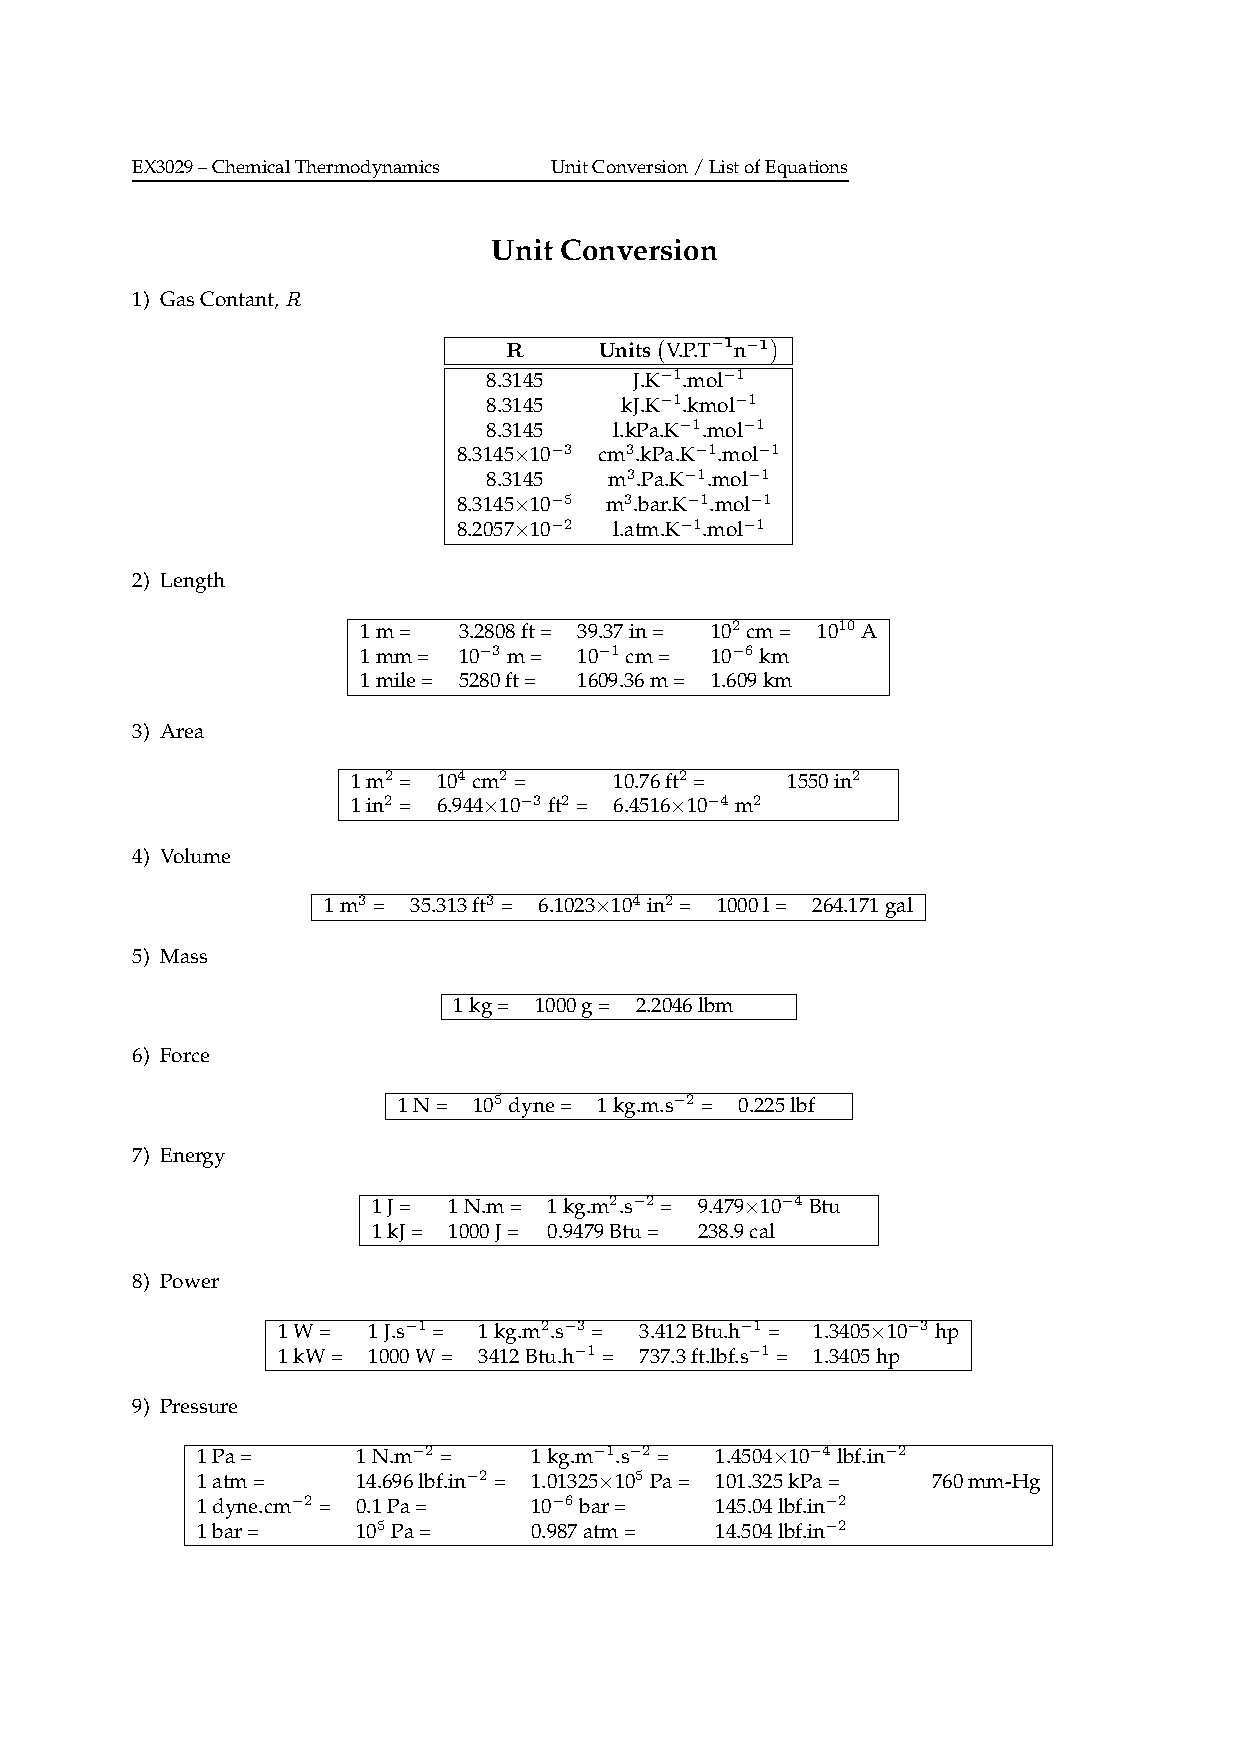
\includepdf[pages=-,fitpaper]{./Pics/EquationsList}
}
%\end{comment}



\end{document}
